
\section{Introduction}
Causal reasoning is important because scientific, medical, and policy decisions depend on how systems would respond to interventions, not only on observed associations \citep{Pearl_2009,pearl2018why,imbens_rubin_causal_2015}.
Yet measuring and making progress in causal reasoning remains challenging, particularly for today's large language models (LLMs).
Existing benchmarks generally
 translate causal graphs, datasets, or narratives into question-answering and classification tasks \citep{qin2019counterfactual,romanou2023crab,stolfo2023causal,jiang2024can,vashishtha2025teachingtransformerscausalreasoning,jin2024cladderassessingcausalreasoning,wang-2024-causalbench,clear2024,corr2cause2024}.
While useful, they leave open the ``causal parrot'' concern \citep{zecevic2023causal}:
models can succeed with memorized causal facts or linguistic cues rather than causal reasoning behaviors needed to discover causal mechanisms \citep{zheng2023preservingcommonsenseknowledgepretrained,liu2023kept}.

\begin{figure*}[t]
\centering
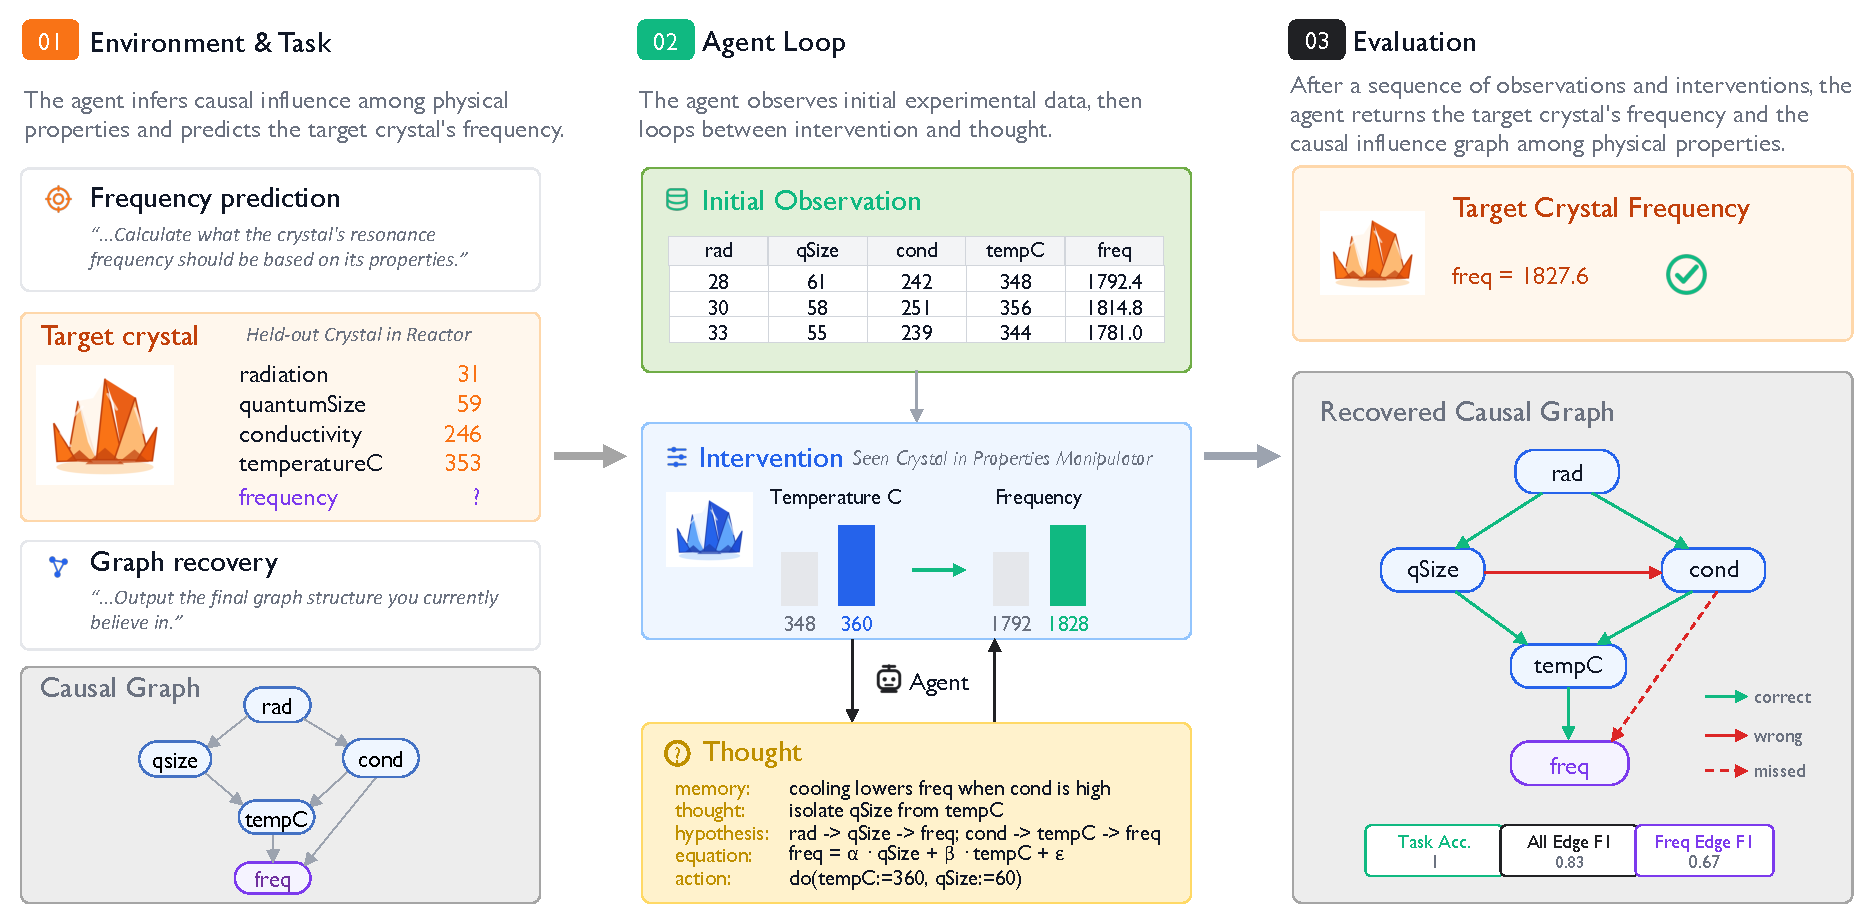
\includegraphics[width=1.0\linewidth]{figures/main_figure_20260517_junlin.pdf}
\caption{Overview of a \projectname{} episode. \textbf{(1)} A hidden SCM generates prior records, a manipulator crystal, and a held-out reactor crystal. \textbf{(2)} The agent observes records and performs budgeted interventions on the manipulator crystal. \textbf{(3)} At each step it emits a DSL thought parsed against the ground-truth SCM. \textbf{(4)} It predicts the reactor \texttt{frequency}; we score both the prediction and recovered-mechanism trajectory.}
\label{fig:causal_main}
\end{figure*}

To illustrate, let's consider the following thought experiment. Suppose we are interested in studying the causal relationship between temperature and the resonance frequency of a crystal. An LLM agent might appear useful in at least two different ways. (1) It may retrieve from existing sources, such as Wikipedia or its training data, that temperature causes resonance frequency.
(2) It may observe paired measurements of temperature and frequency, formulate hypotheses, design experiments, perform interventions, observe the resulting changes, and infer causation from evidence \citep{Pearl_2009,JMLR:v13:hauser12a,lampinen2023passive}. While both are valuable in practice, (1) offers little help when the relevant causal knowledge lies beyond the current frontier of human knowledge.
We therefore argue that (2) is especially important, particularly for important applications such as scientific discovery, because it enables LLM agents to help advance the frontiers of knowledge in a manner closer to what human scientists would do \citep{langley2019scientific,dunbar_fugelsang_2005,DBLP:journals/corr/abs-2406-06769}.

We introduce \projectname{} (Figure~\ref{fig:causal_main}), a scalable environment for evaluating LLM agents as interactive causal discoverers, joining a recent line of interactive scientific-agent and causal-discovery benchmarks \citep{DBLP:journals/corr/abs-2406-06769,igda2025,chen2026causalgame,chen2025autobench,geng2025reliableaiscientists}. Each episode asks the agent to use evidence from prior records and interventions on one crystal to predict the held-out frequency of another crystal. The shared data-generating mechanism is a hidden structural causal model (SCM) \citep{Pearl_2009}, with a causal graph and structural equations that determine the crystal properties and frequency.
The agent receives prior measurement records, can run budgeted interventions on a manipulator crystal through a property manipulator, and must predict the frequency of a separate reactor crystal governed by the same SCM (Figure~\ref{fig:causal_main}; \S\ref{sec:benchmark}). Two design choices distinguish \projectname{} from prior causal-reasoning evaluations. First, the hidden SCM is sampled per episode rather than drawn from public causal corpora, which sidesteps the ``causal parrot'' concern that scores reflect memorized causal lexicon. Second, a lightweight domain-specific language (DSL; \S\ref{sec:dsl}) records the agent's accumulated evidence, current graph and equation hypothesis, planned experiment, and action at each step, so we can score not only the final prediction but also the trajectory-level faithfulness of the recovered mechanism to the ground-truth SCM (\S\ref{sec:experiments}).

Our experiments span closed and open-weight models, multiple model sizes, and thinking versus non-thinking variants, surfacing four findings that prior static benchmarks cannot reach. \textbf{(1) Correct predictions often do not reflect correct mechanism discovery.} Across matched functional-form controls, hidden-perturbation controls, and target-edge controls, endpoint accuracy and mechanism fidelity move separately: agents can find plausible parents while missing quantitative equations, preserve task success while degrading all-edge recovery, or lose accuracy mainly when the target equation itself is perturbed. \textbf{(2) Observation-conditioned online intervention best balances prediction and graph recovery.} Pure observation can boost endpoint accuracy without recovering structure, and pure intervention is weak before observations narrow the hypothesis space. For \texttt{GPT-5.2-high} on 6-node graphs, pure observation reaches 92\% accuracy but only 0.47 all-edge $F_1$, while mixed online observation--intervention reaches 80\%/0.80. Offline intervention traces do not replace online experimental choice: injecting ``Golden'' chains raises \texttt{GPT-5-mini} accuracy to 90\% on 4 nodes while \emph{lowering} all-edge $F_1$. \textbf{(3) Model family and scale pay off unevenly across the two axes.} \texttt{GPT-5.2-high} has the best endpoint accuracy and lowest directed all-edge structural Hamming distance (SHD) at every graph size, but gains are not uniform across graph sizes or metrics. Open-weight \texttt{Qwen3.5} can approach \texttt{GPT-5-mini} on some task scores, yet its SHD rises faster as graphs grow; thinking generally lowers Qwen SHD. Even \texttt{GPT-5.2-high} drops to 64\% accuracy and directed SHD 4.761 at 7 nodes. \textbf{(4) Many failures come from premature commitment, not exhausted budget.} Both successful and failed runs leave roughly half the intervention budget unspent, failed runs end with hypotheses inconsistent with their own data, and a single explicit verification step lifts 4-node accuracy from 48\% to 60\%. \projectname{} therefore separates predictive success from causal understanding, revealing how current LLM agents still struggle to explore unfamiliar environments interactively, test candidate mechanisms, and revise toward the causal regularities that govern them.

